% Some commands used in this file
\newcommand{\package}{\emph}

\chapter{Introduction}

\section{Motivation}

Modern image techniques are rabidly becoming less noisy, less expensive and higher resolution especially in Biology and Medicine. This large array of different imaging techniques is producing an ever increasing volume of high dimensional data which is impossible for humans to analyse without computer assistance. Particularly for three dimensional data humans have difficulty using their normal spacial reasoning as the images can not truly be displayed in three dimensions because one needs to look through the tissues to see the relevant markers and hence humans must resort to analysing the images in a series of two dimensional slices \cite{denk2004serial}, \cite{megason2007imaging}, \cite{keller2008reconstruction}, \cite{peng2011brainaligner}. To Service researchers working with three dimensional data we are creating an open-source distributed framework for 3d image segmentation that can be easily adopted to many data types. 

\section{Image Segmentation as Structured Prediction}
Structured Prediction is a subset of supervised machine learning which solves problems where the output variable can not be represented as a simple label or scalar value. In our applications we are attempting image segmentation which in a naive implementation could be modelled as massively single nominal variable classification problem where each pixel is assigned a feature vector but the spatial relation between pixels is not considered.  While the classification groundtruth is per pixel we are interested in the true objects which originally produced these pixels and their relations to other objects in the visible field. Hence the problem is more accurately modelled as joint classification problem over all pixels in the image. We structure image segmentation as conditional random field of groups of pixels which are have edges to their spatially adjacent groups. These groups of pixels can also be called super-pixels.
\begin{figure}
  \centering
  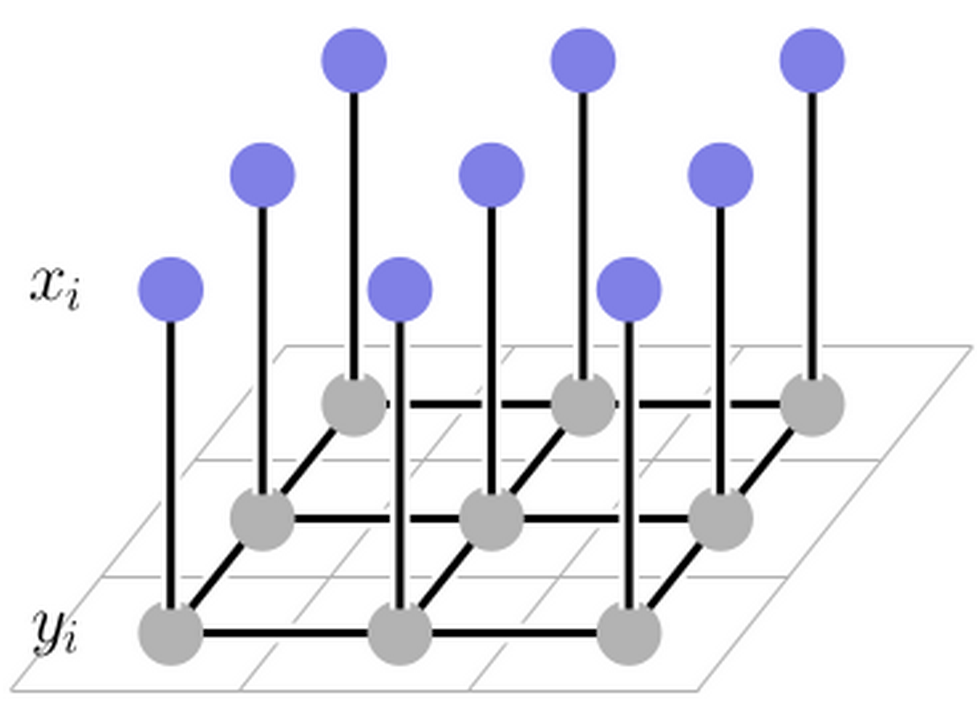
\includegraphics[width=0.7\textwidth,natwidth=610,natheight=642]{images/crfImage.png}
  \caption{Visualization of a Conditional random field for image segmentation where $y_i$ are the super-pixel labels, the edges between $y_i$ are the pairwise potentials, $x_i$ are the unary features of that super pixel and the edges between $x_i$ and $y_i$ are the unary potentials} 
  \label{fig:crfgraphic}
\end{figure} 

\par  More specifically the conditional random field has 1 node per super-pixel representing its label which has a unary potential linked to its unary-feature node and a pairwise potential linked to each of its neighbours. Considering each pixel a part of a joint output domain results in an output space of $K^n$, where $K$ is the number of possible labels and $n$ is the number of pixels or super-pixels. Due to this large domain standard classification methods will not work, in this paper we take the Structured Support Vector Machine (SSVM) approach. 
\section{The Pipeline}
For color or grayscale 3D tif stacks image data super-pixels are constructed with the Simple Linear Iterative Clustering (SLIC) algorithm. The super-pixel to pixel assignment mask is then used to construct a graph where each node receives a feature vector calculated from only the pixels assigned to this super-pixel. The ground truth is transformed into a graph with the same mask by assigning each node the label which the majority of its pixels have. This training dataset is then used to learn an SSVM with Block Coordinate Frank-Wolfe  (BCFW). The training occurs in equal partitions locally on different machines; at the end of every round the accumulated weights are recombined by the master node. Each the executor machines find the most constraining possible next update direction, this sub-problem is called the max-oracle. We implemented Mean Field to perform the max-oracle step but also included Loopy Belief propagation from the factorie package\cite{mccallum09:factorie:}.  The moving of data and managing computational resourches is done through the SPARK framework\cite{spark} with the CoCoA algorithm, which is designed to reduce lower network traffic. CoCoA and the BCFW solver is taken from the dissolve-struct framework \cite{dissolvestructWeb}. Once training is completed the model is again synchronized on the executor node and prediction is performed on the test dataset. 

\todo{Add image showing. Original Image, Super-pixel Boundaries,real ground truth, Ground truth interms of super pixels, a graph with labels and features, some image representaing and SVM, and then predicted outcome again interms of pixels} 

\section{Compare To other work}

For the super-pixel preprocessing step of our pipeline we choose to use SLIC super-pixels because of its time complexity and ability to control the number and shape regularity of the resulting super-pixels. Regularity of super-pixels in space is important to our model because it does not retain any information about the original spacial relations between pixels except for which super-pixels where neighbours during preprocessing. For the SSVM solver we chose BCFW because it can be distributed over $n$ machines if the dataset has $n$ training examples and has good convergence properties even with approximate max-oracle solvers \cite{lacoste2012block}.
\subsection{Super-pixel Alternatives}
One group of alternative super-pixel generation algorithms are graph based. Where in each pixel is initially considered to be a single node in a graph with undirected edges to its adjacent pixels. The edges are assigned weights based on a feature map including information from both neighbours member pixels. Then standard graph processing algorithms are used to minimize a global energy function over this graph resulting in a disconnected graph of super-pixels. 
One such algorithm is the Normalized cuts algorithm \cite{shi2000normalized}. The global criteria, defined by normalized cut, captures information of total dissimilarity between node grouping and also total similarity within the groups. The segmentation algorithms based on this criteria can achieve a computational complexity of $\mathcal{O}(N^{\frac{3}{2}})$ \cite{levinshtein2009turbopixels}. While the algorithm has had some success \cite{mori2005guiding} we prefer SLIC for 3D images due to its lower complexity of $\mathcal{O}(N)$. 
\par
Another graph approach was proposed by Fezenszwalb and Huttenlocher \cite{felzenszwalb2004efficient} which performs well with images that include both high variance and low variance regions. The algorithm performs global clustering where each super-pixel is the smallest spanning tree to cover its pixels. This approach has a better time complexity of $\mathcal{O}(N\log N)$ but in contrast to SLIC it does not have the ability to control the number of super pixels or the regularity of their shapes. 
\par 
A non parametric approach was introduced by Comaniciu and Meer which performs a recursive mean shift in the direction of the nearest stationary point of an underlying density function to find the mode of the distribution \cite{comaniciu2002mean}. It has been shown that this algorithm is equivalent to the Nadaray-Watson regression kernel. Again this algorithm does not have the ability to control the number or shape of the resulting super-pixels. 
\par
An empirically faster mode seeking algorithm, Quick Shift, was introduced in 2008 \cite{vedaldi2008quick}. The algorithm, for each pixel, finds the closest pixel in terms of increasing the Parzen density estimator and then moves them together. While it is quiet fast this algorithm also can not control the number or compactness of the resulting super-pixels. 

\subsection{SSVM Solver Alternatives}

The most common way of solving SVMs are the stochastic gradient descent algorithms (SGD). The direct generalization if SGD for problems with objective functions which are not differentiable, the stochastic sub-gradient descent algorithm (SSGD), has found some applications in structured learning \cite{ratliff2007approximate} \cite{tsochantaridis2005large} \cite{roller2004max}. Stochastic sub-gradient descent has a good convergence rate of $\tilde{O}(\frac{1}{\varepsilon})$ and like BCFW only requires on max-oracle call. But SSGD applies line search to an objective that is not differentiable may result in convergence to a suboptimal point. To avoid this problem and actually achieve the stated convergence rate it is assumed the user has specified an appropriate sequence of step sizes for the given problem \cite{ratliff2007approximate}. This additional tuning parameter of the step-size sequence is not required for BCFW because we can calculate the optimal step-size per iteration. 

\subsection{Alternative Software Packages}
NiftySeg is a 3D Image segmentation framework targeting brain imagery. It uses EM based segmentation with good performance on their data. Another valuable portion of the framework are the features specially designed for MRI images\cite{cardoso2011niftyseg}. NiftySeg is a very useful tool in its specific field of application but as it is not a distributed system the size of the datasets it can reasonably process are limited. 
\par
Another specialized open-source framework was published in 2013 named NIRFAST \cite{jermyn2013fast}. It is specialized for MRI images and utilizes blood oxygen saturation, water content and lipid concentration to construct the image segments. But again this framework was not designed to run on a distributed system. 